% META: DONE.1

\section{Эволюция архитектурного подхода}

\subsection{Прямое предсказание API: наивный подход}
На начальном этапе исследования была предпринята попытка обучить нейросеть напрямую генерировать текстовую команду, напрямую соответствующую вызову API КОМПАС-3D, по двум соседним состояниям геометрии (начальная и конечная модель). Для этого использовалась архитектура на основе DGCNN для извлечения признаков из двух облаков точек, отвечающих за две модели отличающихся одни атомарным шагом построения, и одной LSTM для генерации последовательности токенов (рисунок \ref{fig:naive-pointcloud-architecture}).

\begin{figure}[h]
    \centering
    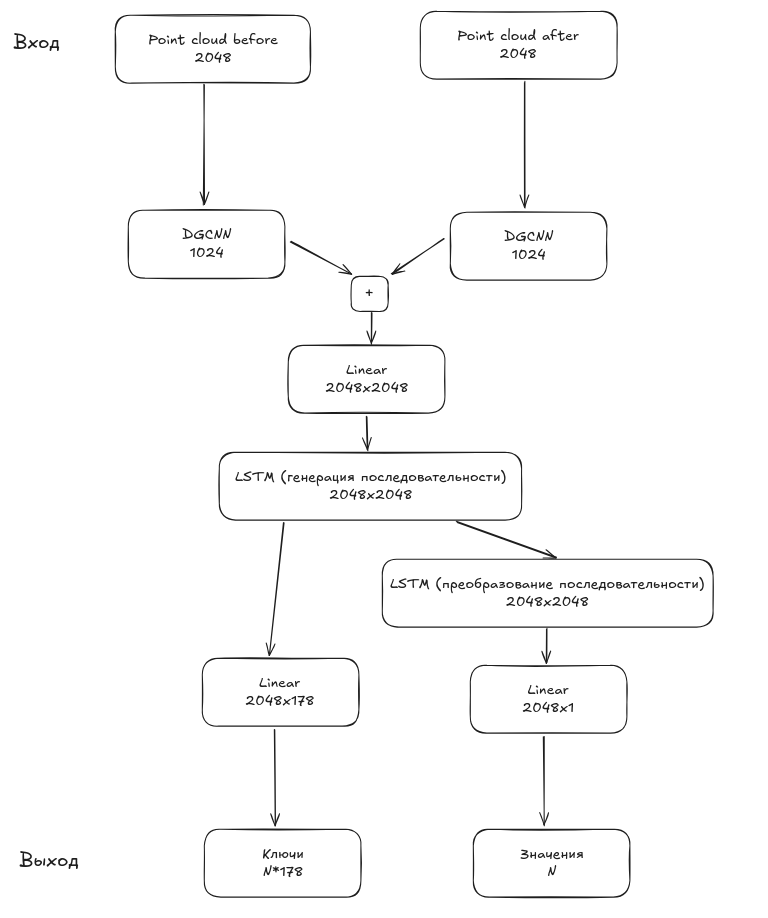
\includegraphics[width=0.8\linewidth]{figures/naive_pointcloud_architecture.png}
    \caption{Архитектура наивного подхода}
    \label{fig:naive-pointcloud-architecture}
\end{figure}

Эксперименты показали, что сеть успешно определяет \textbf{тип} операции (выдавливание, вырезание, скругление, фаску), а также подстраивается под формат API и выдаёт корректные названия параметров в верной последовательности в более чем 49.7\% случаев. Однако, различные операции требуют совершенно различных параметров, поэтому нейронная сеть подстраивалась под самые часто встречаемые операции и последовательности, а нерепрезентативные последовательности параметров практически игнорировались.

\subsection{Прямое предсказание API: модульная архитектура}
Для смягчения проблемы была предложена двухэтапная архитектура: сначала классификатор определял тип операции, а затем специализированный регрессионный блок предсказывал параметры уже конкретной операции (рисунок \ref{fig:naive-modular-architecture}).

\begin{figure}[h]
    \centering
    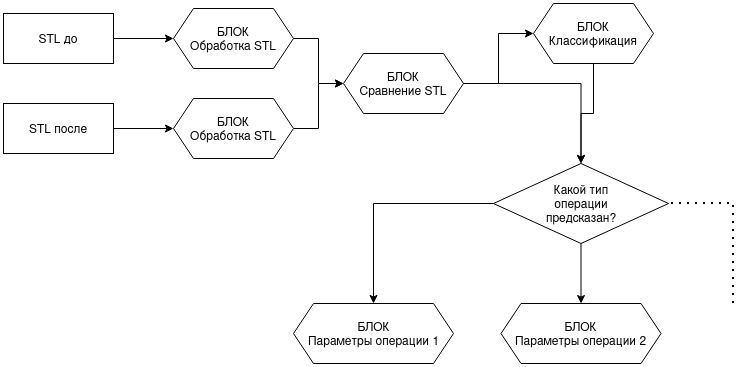
\includegraphics[width=0.8\linewidth]{figures/naive_modular_architecture.png}
    \caption{Верхнеуровневая архитектура модульного подхода}
    \label{fig:naive-modular-architecture}
\end{figure}

Классификатор работал на основе сравнения двух облаков точек (конкатенация эмбеддингов), а регрессоры были реализованы как отдельные небольшие сети, принимающие на вход разность геометрических признаков. Качество классификации удалось повысить до 90\% для некоторых операций, но регрессия параметров (глубина, радиус, координаты) по-прежнему оставалась узким местом. Причина - высокая чувствительность к системе координат и дискретизации: даже ошибка в 1-2\% от масштаба модели в единственном параметре может привести к невалидной геометрии при попытке воспроизвести операцию в КОМПАС-3D (например, ошибка в одной координате сложного контура, делающего контур незамкнутым).

Пример одной из подобных команд API (скругление по квадратному контуру):

{
\small
\begin{lstlisting}
...
Step4 
Feature = o3d_cutExtrusion 
Extrusion = Angle_NormalTrue = 0.000 AngleDirection_NormalTrue = False \
  Angle_NormalFalse = 0.000 AngleDirection_NormalFalse = False \
  Depth_NormalTrue = 131.000 Depth_NormalFalse = 0.000 Direction = 0 \
  Thin = False ThinType = 2 Thickness_NormalTrue = 0.000 \
  Thickness_NormalFalse = 0.000 Cut = True 
Sketch = Angle = 0.0000000 Direction = 0 LeftHandedCS = 0 
o3d_face Face = X = 8.040 Y = -38.833 Z = 42.000 
LineSegment = X1 = -10.11 Y1 = 52.42 Length = 49.00 Angle = 0.00 Style = 1 
LineSegment = X1 = 38.88 Y1 = 52.42 Length = 38.00 Angle = 270.00 Style = 1 
LineSegment = X1 = 38.88 Y1 = 14.42 Length = 49.00 Angle = 180.00 Style = 1 
LineSegment = X1 = -10.11 Y1 = 14.42 Length = 38.00 Angle = 90.00 Style = 1 
...
\end{lstlisting}
}
Здесь отрезки задаются с помощью координат одного из концов в локальной системе кооординат выбранной грани, после чего указывается его направление (угол) и длина. Все эти параметры особенно чувствительны к малейшим измененениям, приводя к деформации контура или к невалидным параметрам операции. Дальнейшее продвижение в данном направлении требовало бы уточнение, улучшение и упрощение формата описания API, например переход в глобальную систему координат и привязка контуров к вершинам вместо описания каждого отрезка независимо.

\subsection{Гибридный подход: сегментация + детерминированное CAD-вычисление}
Ключевым поворотным моментом стало переосмысление роли нейросети. Вместо того чтобы требовать от неё точного численного вывода, было решено возложить на нейросеть задачу локализации следов операции (семантическая сегментация), а точные параметры вычислять детерминированными алгоритмами CAD-ядра на основе B-Rep представления (STEP). Такой подход имеет следующие преимущества:

\begin{itemize}
    \item Нейросеть оперирует в пространстве геометрических паттернов, где она действительно сильна.
    \item CAD-ядро обеспечивает высокую точность и верификацию гипотез.
    \item Результат сегментации интерпретируем (раскрашенная модель), инженеры могут легко визуально оценить результат.
    \item Система может работать итеративно, постепенно упрощая модель.
\end{itemize}

В рамках этого подхода были обучены отдельные классификаторы и сегментаторы для каждой из четырёх операций. Сравнение подходов приведено в таблице \ref{tab:approach-comparison}.

\begin{table}[h]
\centering
\begin{tabular}{|p{4cm}|p{4cm}|p{4cm}|p{3cm}|}
\hline
\textbf{Подход} & \textbf{Преимущества} & \textbf{Ограничения} & \textbf{Итоговая оценка} \\
\hline
Прямое предсказание команд API & Явный формат выхода; логичная интеграция через API & Высокая чувствительность к численным параметрам, системе координат и накоплению ошибки & Хорошая исследовательская гипотеза, но недостаточно устойчива \\
\hline
Модульная классификация + регрессия & Разделение типа операции и параметров; расширяемость по операциям & Параметры остаются труднорегрессируемыми из дискретизированной геометрии & Ценный промежуточный шаг \\
\hline
Гибридный: сегментация + CAD & Соответствует природе 3D-данных; интерпретируемый результат; перенос точных вычислений в CAD & Требует автоматической разметки и балансировки датасета & Наиболее перспективный подход (реализован) \\
\hline
\end{tabular}
\caption{Сравнение подходов к реализации}
\label{tab:approach-comparison}
\end{table}

